% Seção de Metodologia
\section{Formalização e Modelagem do Problema}

% \begin{frame}{Formalização do Problema}

%     \begin{block}{Definição}
%     \begin{itemize}
%         \item Construção de uma agenda de atendimentos entre paciente e médico \cite{Canter_1977}
%         \item Construir uma agenda acíclica e justa para enfermeiras \cite{Fitzpatrick_Farrell_Richter_Zeunik_1987}.
%     \end{itemize}

%     \end{block}

%     \vspace{3cm}
% \end{frame}

\begin{frame}{Formalização do Problema}

    \begin{block}{O que é pedido do problema...}
            Construir a agenda de trabalho de múltiplas unidades para todos os médicos
    \end{block}

    \begin{figure}
        \centering
        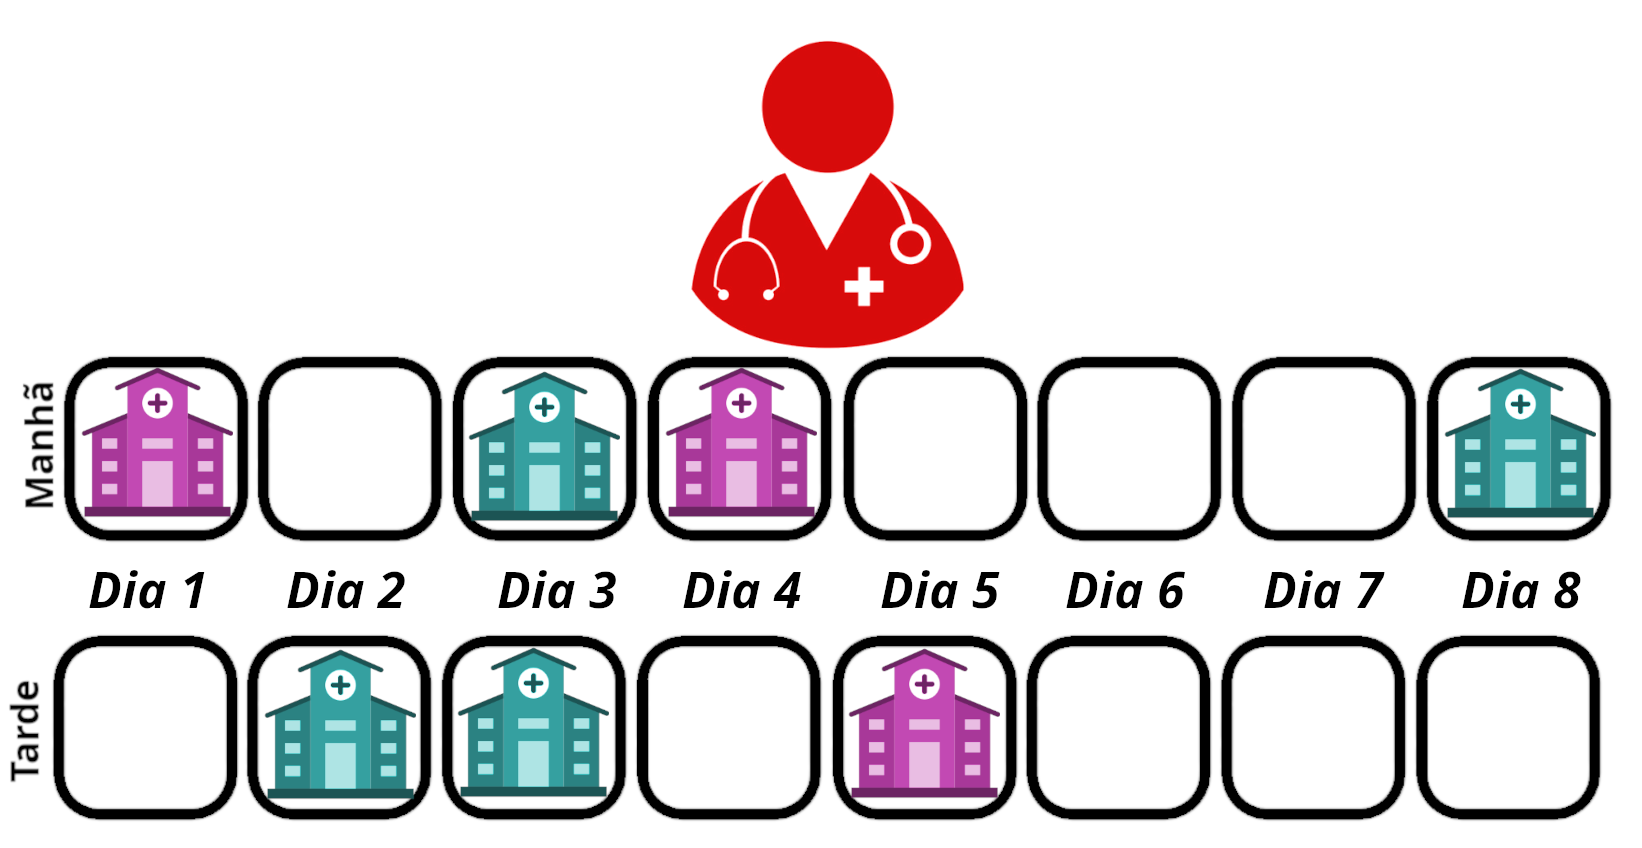
\includegraphics[width=0.5\linewidth]{img/exemplo-schedule-medico.png}
        \caption{Exemplo de agenda de um médico}
        \label{fig:enter-label}
    \end{figure}
\end{frame}

% \begin{frame}{Informações do Cenário}

%     \begin{block}{Alguns dados são previamente estabelecidos}
%         \begin{itemize}
%             \item Demanda
%             \item Disponibilidade de atendimentos
%             \item Salas disponíveis
%         \end{itemize}
%     \end{block}

% \end{frame}

\begin{frame}{Componentes do Problema}
    \begin{small}
	\begin{longtable}[l]{lllll}
		\multicolumn{5}{l}{\textbf{Índices e conjuntos}}    \\
		$i \in I$ \quad & Médicos & \quad & $t \in T$ \quad & Turnos  \\
		$u \in U$ \quad & Unidades & \quad & $I_u$ \quad & Médicos que atendem na unidade $u$ \\
		$d \in D$ \quad & Dias & \quad & $U_i$ \quad & Unidades atendidas pelo médico $i$\\ 
	\end{longtable}

	\begin{longtable}[l]{ll}
		\multicolumn{2}{l}{\textbf{Parâmetros}}    \\
		$e_{udt}$       \quad   & Demanda por exames na unidade $u$ no dia $d$ e turno $t$ \\
		$s_{ut}$       \quad   & Salas disponíveis para exames na unidade $u$ no dia $d$ e turno $t$ \\
		$q_{idt}$      \quad   & Quantidades de exames que o médico $i$ pode realizar dia $d$ e turno $t$ \\
		$a_{idt}$      \quad & Disponibilidade de trabalho do médico $i$ no dia $d$ e turno $t$   
        % &  $\begin{cases} 1, & \text{se o médico $i$ estiver disponível para trabalho no dia $d$ e turno $t$} \\
			% 0, & \text{caso contrário.}\end{cases} $ \\
   %  	$b_{udt}$      \quad   &  $\begin{cases} 1, & \text{se a unidade $u$ tem demanda no dia $d$ e turno $t$} \\
			% 0, & \text{caso contrário.}\end{cases} $
	\end{longtable}

    \begin{longtable}[l]{ll}
		\multicolumn{2}{l}{\textbf{Variáveis}}    \\
		$x_{iudt}$ \quad & Variável binária para alocação do médico $i$ na clínica $u$ no dia $d$ e turno $t$ \\
		$w_{iud}$ \quad  & Variável binária para alocação do médico $i$ na clínica $u$ no dia $d$ \\
		$c_{udt}$  \quad & Exames não atendidos na clínica $u$ no dia $d$ e turno $t$ \\
		$z_{id}$   \quad & Variável binária indicando se o médico $i$ trocou de clínica no dia $d$   
        \end{longtable}
    \end{small}
\end{frame}

\begin{frame}{Modelagem Matemática}
\resizebox{\textwidth}{!}{\begin{minipage}{1.3\textwidth}

        % EQ pre processamento
        \begin{block}{Impedir Alocação em Clínicas Não Associadas}
            \begin{alignat}{2}
                w_{iud} = 0 \quad & \forall i \in I, u \notin U_i, d \in D
            \end{alignat}
        \end{block}

        % EQ Alocação por disponibilidade
        \begin{block}{Alocação por Disponibilidade}
            \begin{alignat}{2}
                \sum_{u \in U_i} x_{iudt} \leq a_{idt} & \quad \forall i \in I, d \in D, t \in T
            \end{alignat}
        \end{block}

        
        \begin{block}{Restringir remanejamento entre turnos}
            \begin{alignat}{2}
                \sum_{u \in U_i} w_{iud} \leq 1 & \quad \forall i \in I, d \in D \\
    	    x_{iudt} \leq w_{iud} & \quad \forall i \in I, u \in U, d \in D, t \in T
            \end{alignat}
        \end{block}

\end{minipage}}
\end{frame}

\begin{frame}{Modelagem Matemática}
\resizebox{\textwidth}{!}{\begin{minipage}{1.3\textwidth}

        % EQ pre processamento
        \begin{block}{Alocação sob Capacidade das Clínicas}
            \begin{alignat}{2}
               \sum_{i \in I_u} x_{iudt} \leq s_{udt} \quad & \forall u \in U, d \in D, t \in T \label{eq:r5}
            \end{alignat}
        \end{block}

        % EQ Alocação por disponibilidade
        \begin{block}{Garantir Cobertura Mínima}
            \begin{alignat}{2}
               \sum_{i \in I_u}x_{iudt} \geq 1 \quad & \forall u \in U, d \in D, t \in T \label{eq:r6}
            \end{alignat}
        \end{block}

        
        \begin{block}{Domínio das Variáveis de Decisão}
            \begin{alignat}{2}
                x_{iudt}, w_{iud} \in \{0,1\} \quad & \forall i \in I, u \in U, d \in D, t \in T \label{eq:dom2}
            \end{alignat}
        \end{block}

    % \end{alignat}

\end{minipage}}
\end{frame}

\begin{frame}{FO1 - Minimização de Exames Não Atendidos}

\resizebox{\textwidth}{!}{\begin{minipage}{1.2\textwidth}

\begin{block}{Motivação}
Funcionalidade da operação.   
\end{block}

\vfill


    \begin{equation} 
    	\min \sum_{u \in U}\sum_{d \in D}\sum_{t \in T} c_{udt} \label{eq:fo1-fo}
    \end{equation}
    \hspace{1.5cm} sujeito à:
    \begin{alignat}{2}
	c_{udt} \geq e_{udt} - \sum_{i \in I_u}(q_{iut} \cdot x_{iudt}) \quad & \forall u \in U, d \in D, t \in T \label{eq:fo1-r1} \\
	c_{udt} \in \mathbb{Z}^{*}_{+} \quad & \forall i \in I, u \in U, d \in D, t \in T \label{eq:c-domain}
\end{alignat}

\end{minipage}}
\end{frame}

\begin{frame}{FO2 - Minimização de Trocas}

\resizebox{\textwidth}{!}{\begin{minipage}{1.3\textwidth}

\begin{block}{Motivação}
Ergonomia no serviço.
\end{block}

    \begin{figure}
        \centering
        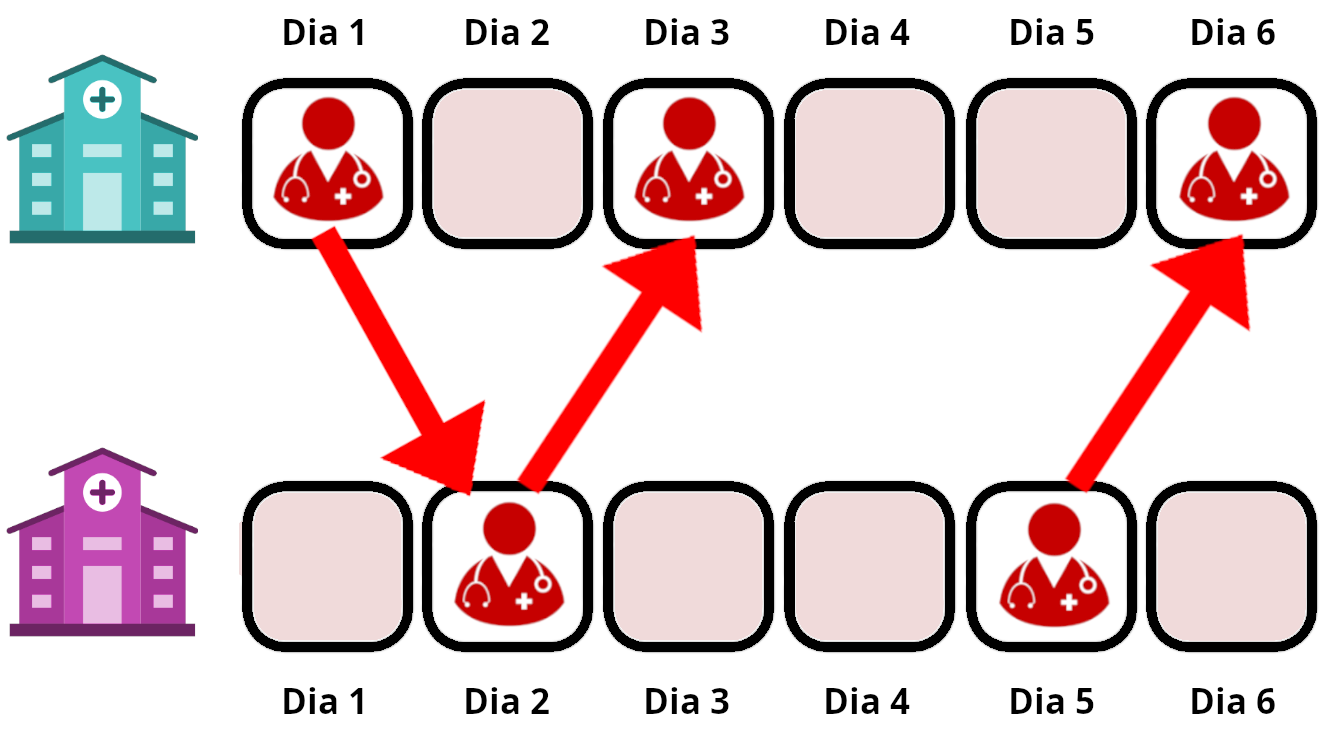
\includegraphics[width=0.6\linewidth]{img/troca-examplo.png}
        \caption{Exemplo de trocas em uma agenda}
        \label{fig:enter-label}
    \end{figure}
        
\end{minipage}}
    

\end{frame}

\begin{frame}{FO2 - Minimização de Trocas}

\resizebox{\textwidth}{!}{\begin{minipage}{1.3\textwidth}

    \begin{block}{Motivação}
        Ergonomia no serviço.
    \end{block}
        
    \begin{equation} 
    	\min \sum_{i \in I}\sum_{d \in D} z_{id} \label{eq:fo2-fo}
    \end{equation}
    \hspace{1.5cm} sujeito à:
    \begin{alignat}{2}
    	z_{id} \geq (w_{iud} + \sum_{u' \neq u}^{U} w_{i,u',d-1}) - 1 \quad & \forall i \in I, u \in U, d \in D - \{1\} \label{eq:fo2-r1}  \\
            z_{id} \in \mathbb{B} \quad & \forall i \in I, d \in D
    \end{alignat}
\end{minipage}}
    

\end{frame}

\begin{frame}{FO3 - Hierárquica}

    \begin{block}{}
        É possível obter uma solução considerando o compromisso entre as duas funções objetivos?
    \end{block}

    \vspace{5cm}

\end{frame}

\begin{frame}{FO3 - Multiobjetivo}

    \begin{block}{}
        É possível obter uma solução considerando o compromisso entre as duas funções objetivos?

        
    \end{block}
    \vspace{1cm}
    \begin{figure}
        \centering
        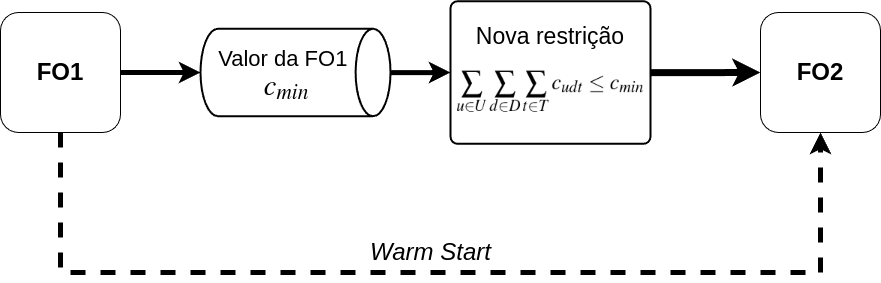
\includegraphics[width=1\linewidth]{img/fo3-diagrama.png}
        \caption{Função Objetivo Multiobjetivo}
        \label{fig:enter-label}
    \end{figure}

\end{frame}